\chapter{Theoretische Grundlagen}
    \section{Schach}
   Schach ist ein strategisches Brettspiel für zwei Spieler, welches auf einem quadratischen Spielfeld mit 64 Feldern gespielt wird. Jeder Spieler beginnt mit 16 Figuren und das Ziel des Spiels ist es, den König des Gegners schachmatt zu setzen, indem man ihn bedroht, ohne dass der Gegner den Angriff verhindern kann. 
   
   Wie Figuren sich bewegen und andere Figuren schlagen erkläre ich nicht explizit, lediglich zwei Sonderregeln des Schachs und Schachuhren werde ich genauer erklären, da diese bei der Umsetzung des Spiels gesondert gehandhabt werden müssen.
   
   Die erste ist die so genannte \textit{en passant}-Regel. Dabei ist es einem Bauern möglich einen gegnerischen Bauer diagonal zu schlagen, falls dieser zwei Felder gezogen ist und nun auf der gleichen Höhe wie der eigene Bauer steht (siehe Abbildung \ref{fig:en-passant}).
   
   Die zweite Zusatzregel ist die \textit{Bauernumwandlung}. Sie besagt, dass falls ein Bauer die gegnerische Grundreihe erreicht, dieser Bauer in eine Dame, einen Springer, einen Turm oder einen Läufer umgewandelt werden kann (siehe Abbildung \ref{fig:promotion}).
   
     \begin{figure}[ht]
\raggedleft
  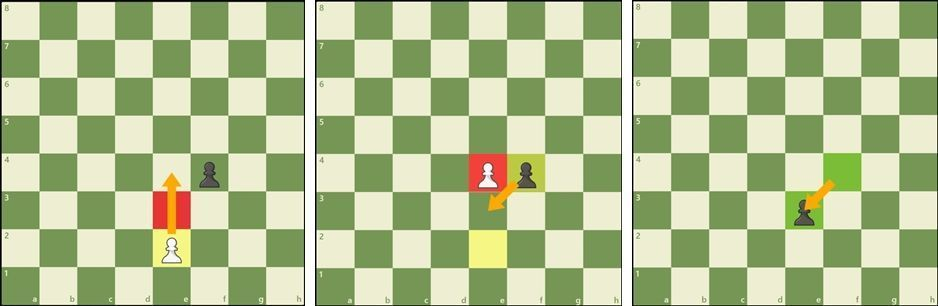
\includegraphics[width=\textwidth]{en-passant.jpeg}
    \footnotesize\sffamily\textbf{Quelle:} \url{https://www.chess.com/de/schachregeln}
  \caption{Die Zusatzregel \textit{en passant}}
  \label{fig:en-passant}
\end{figure}

  \begin{figure}[ht]
\centering
  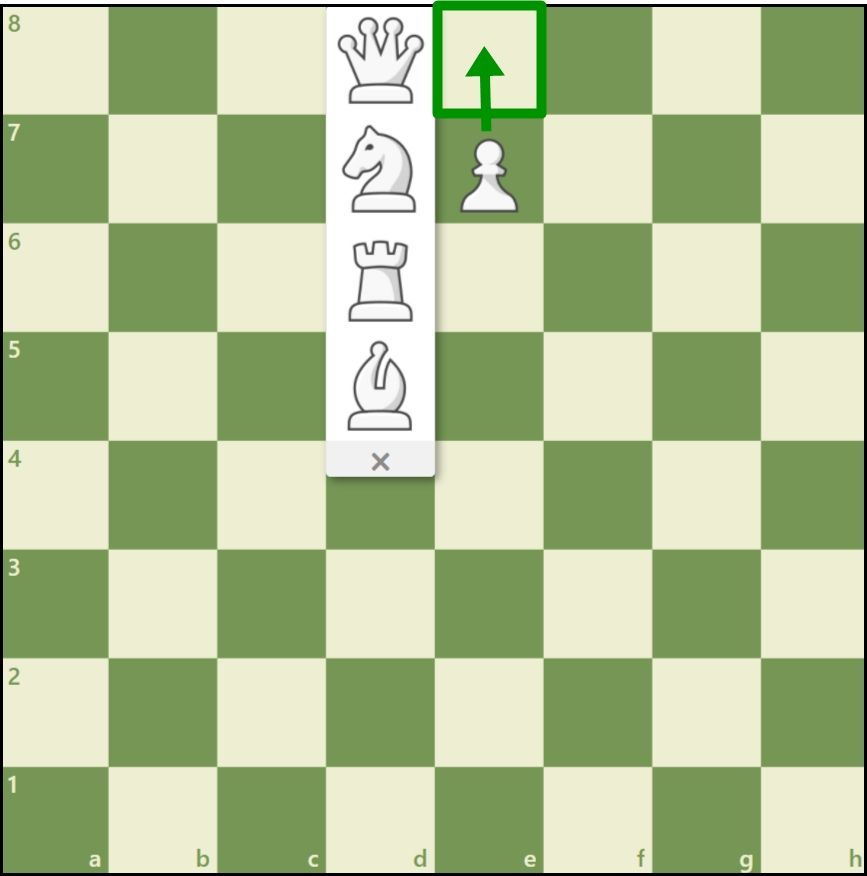
\includegraphics[height=0.4\textwidth]{promotion.jpeg}
   
   
\raggedleft
    \footnotesize\sffamily\textbf{Quelle:} \url{https://www.chess.com/de/schachregeln}
  \caption{Die Zusatzregel \textit{Bauernumwandlung}}
  \label{fig:promotion}
\end{figure}

Die Notation von Schachuhren besteht aus zwei Zahlen, die mit einem Plus getrennt werden, wie zum Beispiel \glqq 10 + 5\grqq .  Hier steht die erste Zahl, in diesem Fall 10, für die Gesamtzeit, die jedem Spieler zur Verfügung steht, also 10 Minuten. Die zweite Zahl, hier 5, wird als Inkrement bezeichnet. Dies bedeutet, dass nach jedem Zug eines Spielers diesem Spieler zusätzlich 5 Sekunden hinzugefügt werden. Dadurch haben Partien mit Inkrement mehr Zeit, je mehr Züge gespielt werden.

Bei Online-Schachpartien ist es zusätzlich üblich, eine bestimmte Startzeit für den ersten Zug jedes Spielers verstreichen zu lassen. Dies gewährleistet, dass die Uhren erst zu laufen beginnen, wenn beide Spieler bereit sind und mitbekommen haben, dass das Spiel gestartet wurde.

    \section{Web-Technologien}
        \subsection{Node.js und Express}
        \subsubsection{Node.js und seine Vorteile}
        \label{sec:node.js}
Node.js ist eine JavaScript-Laufzeitumgebung, welche erstmals 2009 angekündigt wurde\footnote{Quelle: \url{https://www.youtube.com/watch?v=EeYvFl7li9E} am 22. April 2023} und speziell für die Entwicklung von skalierbaren Netzwerkanwendungen entworfen wurde \cite{nodejs}. Skalierbarkeit bedeutet, dass mit steigender Benutzeranzahl der Ressourcenverbrauch idealerweise linear steigt. Zu den relevanten Ressourcen von Webanwendungen gehören Rechenleistung, Ein-/Ausgabeoperationen (kurz I/O) und Arbeitsspeicher, wobei Node.js vor allem die Skalierbarkeit von I/O intensiven Anwendungen verbessert \cite{nodejsbook}.
I/O-Zugriffe sind beispielsweise Zugriffe auf Datenbanken, Webservices oder auf das Dateisystem. Node.js setzt dabei vollständig auf asynchrone Zugriffe. Dabei wartet der Thread nicht auf das Ergebnis eines I/O-Zugriffs, sondern führt andere Aufgaben aus, bis das Ergebnis verfügbar ist. Anschließend wird eine zuvor definierte Callback Funktion (siehe Code Snippet \ref{lst:callback}) durchgeführt. Bei einem synchronen Zugriff, wie es bei einigen anderen Laufzeitumgebungen der Fall ist, würde der Thread auf das Ergebnis warten und dieses anschließend weiterverarbeiten, wobei jedoch sein Speicherplatz zum Teil belegt bleibt.\cite{nodejsbook} Die Vorteile hinsichtlich der Skalierbarkeit werden jedoch erst bei einer hohen Anzahl von Zugriffen erkennbar.

\begin{lstlisting}[style=codeStyle, caption={Beispiel einer Callback Funktion \textbf{Quelle: } \cite{nodejsbook}}, label={lst:callback}]
database.query(  "SELECT * FROM user",  function(result) {
result...
});
\end{lstlisting}


Ein weiterer Vorteil der Nutzung von Node.js ist die Nutzung der gleichen Programmiersprache für Frontend und Backend.
In einem Team-Projekt kann das natürlich besonders hilfreich sein, da Kommunikationsbarrieren durch unterschiedliche Programmiersprachen von Frontend und Backend niedriger sind. Natürlich versteht deshalb der Frontend-Entwickler nicht alles was  der Backend-Entwickler macht und umgekehrt, jedoch gibt es eine gemeinsame Grundlage. Neben den Kommunikationsvorteilen ermöglicht die Verwendung von der gleichen Programmiersprache im Frontend und Backend das Teilen von Code. So ist es zum Beispiel möglich Callback Funktionen vom Frontend an das Backend zu senden und dort aufzurufen.

Node.js basiert auf der Verarbeitung von Requests vom Frontend und dem zurück senden von einem Result mittels dem HTTP-Protokoll. Das HTTP-Protokoll verwendet verschiedene Methoden wie GET, POST, PUT und DELETE, um unterschiedliche Aktionen durchzuführen  \cite{expressbook}. Zum Beispiel wird GET zum Abrufen von Informationen verwendet, während POST zum Senden von Daten verwendet wird. Die Art und Weise wie ein Request verarbeitet werden soll ist dabei selbst zu definieren (siehe Abbildung \ref{fig:node-request}). Dabei kann der Request sein, eine bestimmte Seite zu laden, womit dann mit der entsprechenden HTML-Datei geantwortet wird, oder es kann als API genutzt werden, um Beispielsweise Daten einer Datenbank zu übermitteln. Um die Verarbeitung dieser Anfragen weniger komplex zu gestalten gibt es die Erweiterung \textit{Express} für Node.js.

  

  \begin{figure}[ht]
  \centering
  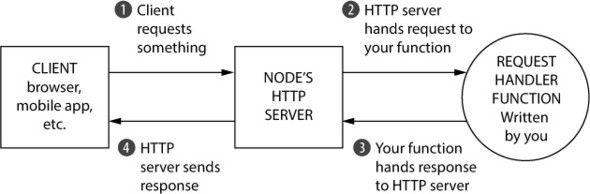
\includegraphics[width=\textwidth]{node-request.jpg}
\raggedleft
    \footnotesize\sffamily\textbf{Quelle:} \cite{expressbook}
  \caption{Ablauf einer Anfrage an einen Node.js Server}
  \label{fig:node-request}
\end{figure}


\subsubsection{Express}
\label{sec:express}
\textit{Express} ist ein leichtgewichtiges und sehr beliebtes Web-Frameworks, welches unter Node.js zur Verfügung steht. Es dient zur Vereinfachung der API von Node.js und stellt hilfreiche Funktionen bereit \cite{expressbook}. Es ermöglicht beispielsweise die Verwendung von \textit{Middleware} und \textit{Routing}.

\textit{Middleware} ermöglicht, dass eine Anfrage an den Node.js Server nicht ausschließlich von einer Funktion bearbeitet werden muss, welche das Ergebnis zurücksendet, sondern von mehreren Funktionen, die sich um verschiedene Teile der Request kümmern (siehe Abbildung \ref{fig:express-request}). Diese Funktionen heißen \textit{Middleware}. Dabei gibt es eine von uns definierte Reihenfolge der Middlewares. Zum Beispiel können wir definieren, dass zu erst der Request von einer Middleware geloggt werden soll, anschließend soll der Benutzer authentifiziert werden und falls der Benutzer eine URL aufrufen möchte, für die er keine Berechtigung hat wird eine \glqq not authorized\grqq{ }Seite zurück gesendet und die nächste Middleware wird nicht aufgerufen. Ansonsten wird die nächste Middleware der Kette ausgeführt, wie zum Beispiel das senden von Informationen (siehe Abbildung \ref{fig:middleware-beispiel}). Ein Vorteil der Nutzung von Middlewares ist, dass es bereits viele vordefinierte Middlewares (auch von Dritten) gibt, welche nützliche Funktionalitäten mitbringen. Die Anfrage des Frontends in mehrere kleinere Funktionen aufzuteilen, anstatt eine Funktion zu schreiben, welche sich um all dies kümmert verringert die Komplexität und erhöht die Modularität.

  \begin{figure}[h]
  \centering
  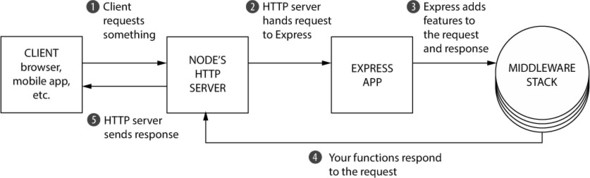
\includegraphics[width=\textwidth]{express-request.jpg}
\raggedleft
    \footnotesize\sffamily\textbf{Quelle:} \cite{expressbook}
  \caption{Ablauf einer Anfrage an einen Node.js Server mit Express}
  \label{fig:express-request}
\end{figure}



  \begin{figure}[h!]
  \centering
  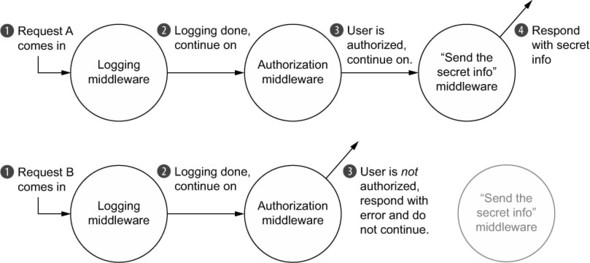
\includegraphics[width=0.7\textwidth]{Middleware-Beispiel.jpg}
  
  \vspace{10mm}
  
  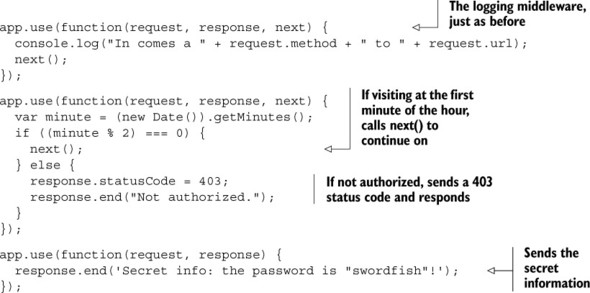
\includegraphics[width=0.7\textwidth]{Middleware-Beispiel-2.jpg}
  
\raggedleft
    \footnotesize\sffamily\textbf{Quelle:} \cite{expressbook}
  \caption{Beispiel der Nutzung von Middlewares}
  \label{fig:middleware-beispiel}
\end{figure}

\textit{Routing} hilft dabei zu identifizieren bei welchem Request welche Middleware ausgeführt werden soll (siehe Abbildung \ref{fig:routing-beispiel}). Beispielsweise kann eine Anfrage an die URL \url{/auth} mit den angegeben Anmeldedaten des Benutzers gesendet werden. Unter diesem Pfad können wir dann bestimmte Middlewares verwenden, welche sich mit der Authentifizierung des Benutzers befassen.

  \begin{figure}[ht]
  \centering
  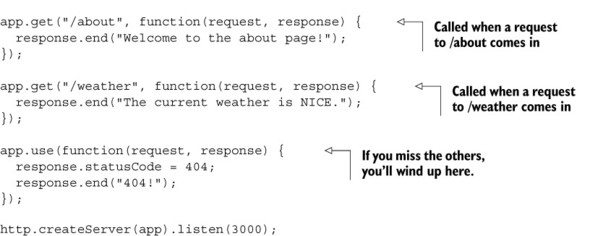
\includegraphics[width=\textwidth]{express-routing-example.jpg}
\raggedleft
    \footnotesize\sffamily\textbf{Quelle:} \cite{expressbook}
  \caption{Beispiel der Nutzung von Routing}
  \label{fig:routing-beispiel}
\end{figure}

        \subsection{Socket.io}
        \label{sec:socket.io}
Die Kommunikation mit dem HTTP-Protokoll über Express hat den Nachteil, dass für jeden Datenaustausch eine neue Verbindung aufgebaut und wieder geschlossen wird, was zu einer Latenz führt, welche für Echtzeit-Anwendungen ungeeignet ist. Diese Problematik behebt das Framework \textit{socket.io}. %QUELLE BENÖTIGT%

Es ermöglicht eine direkte, bidirektionale Echtzeitübertragung von Daten mittels Websockets, long-polling und fünf anderen Protokollen zwischen den Clients und dem Server. Diese Echtzeitkommunikation ist für viele Spiele, wie auch für diese Schach-App, essentiell. So können beim Spielen mit Schachuhr Millisekunden entscheidend sein.
Neben der Echtzeitkommunikation überprüft socket.io unter anderem Timeouts, Verbindungsabbrüche, stellt Verbindungen automatisch wieder her und sorgt dafür, dass die Events in der richtigen Reihenfolge beim Server und beim Client ankommen. 

Die Kommunikation mit Socket.io läuft ausschließlich über Events. So kann man sowohl beim Client, als auch bei dem Server Eventlistener definieren, die auf ein bestimmtes Event hören und darauf hin eine Funktion auf den übertragenen Daten anwenden. Diese Eventlistener (definiert mit der Funktion \verb|.on()|) haben als ersten Parameter den Namen des Events als String, auf den dieser Listener hören soll und als zweiten Parameter die auszuführende Callback Funktion, welche mit den Parametern aufgerufen wird, die beim senden des Events übertragen wurden.

Events können basierend auf verschiedenen Aktionen wie zum Beispiel dem Drücken eines Buttons im Frontend oder als Reaktion eines eingegangenen Events auf dem Server gesendet werden (mit der Funktion \verb|.emit()|) (siehe Abbildung \ref{fig:socket.io-beispiel}). Der erste Parameter der \verb|emit|-Funktion ist wieder der Name des Events als String und im Anschluss kann man beliebig viele Parameter übertragen mit denen die Callback-Funktion des Listeners aufgerufen wird.


  \begin{figure}[ht]
\raggedleft
  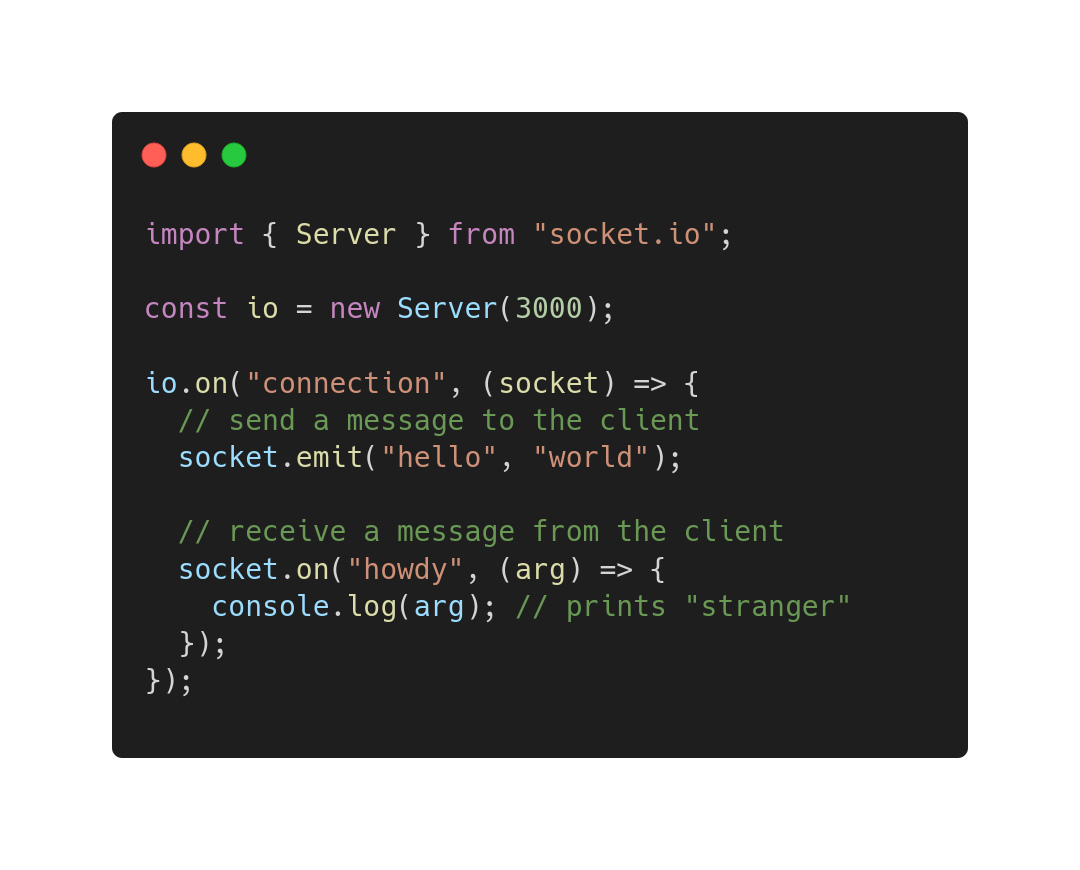
\includegraphics[width=0.45\textwidth]{socket.io-server-beispiel.png}
  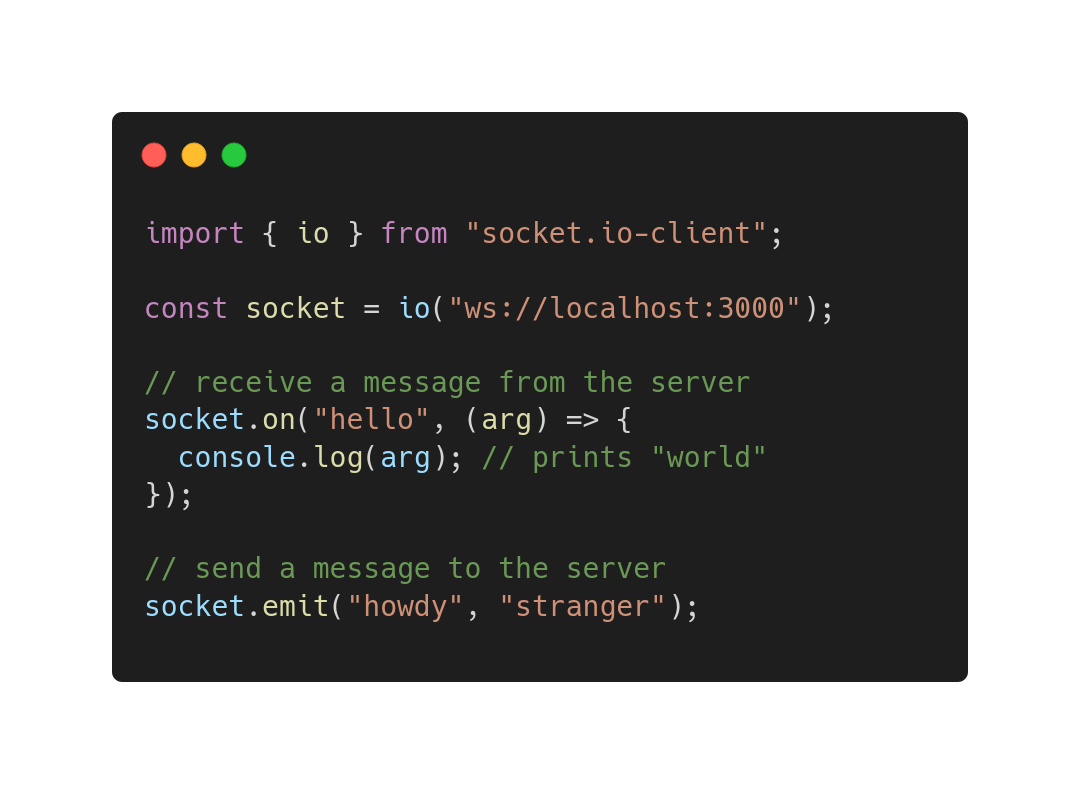
\includegraphics[width=0.45\textwidth]{socket.io-client-beispiel.png}
    \footnotesize\sffamily\textbf{Quelle:} \cite{socketio}
  \caption{Simples Beispiel der Initialisierung einer socket.io Verbindung und das Senden und Empfangen von Events}
  \label{fig:socket.io-beispiel}
\end{figure}

Ein wichtiges Feature von socket.io sind die Räume\footnote{Quelle: \url{https://socket.io/docs/v4/rooms/} am 22. April 2023}. Sockets im Backend können ihnen Beitreten und sie Verlassen. Serverseitig kann man dadurch an alle Sockets, die in einem bestimmten Raum sind etwas senden, ohne es allen einzeln schicken zu müssen (siehe Abbildung \ref{fig:socket.io-room}). Hier kann man sich entschließen das Event an alle clients im Raum zu versenden (\verb|io.to(...).emit(...)|) oder an alle, außer den sender (\verb|socket.to(...).emit(...)|) (siehe Code Snippet \ref{lst:socket-rooms}).


  \begin{figure}[ht]
  \centering
  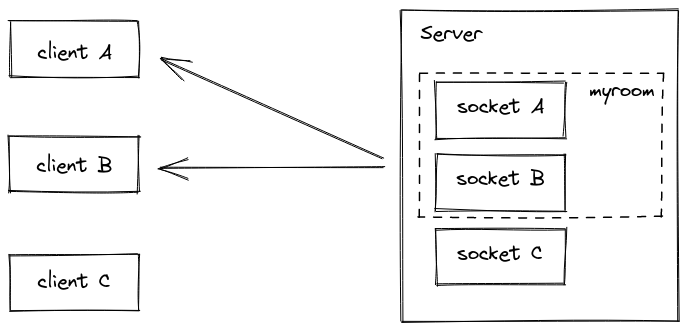
\includegraphics[width=\textwidth]{socket.io-rooms.png}
\raggedleft
    \footnotesize\sffamily\textbf{Quelle:} \url{https://socket.io/docs/v4/rooms/} am 27. April 2023
  \caption{Darstellung eines Raumes \textit{myroom} mit zwei sockets}
  \label{fig:socket.io-room}
\end{figure}

Des weiteren erhält jede socket beim Verbinden eine eigene ID, die ebenfalls als Raum genutzt werden kann. Dementsprechend ist \verb|io.to(socket.id).emit('hello');| äquivalent zu \verb|socket.emit('hello');|.

Socket.io unterstützt wie Express Middlewares, welche bei einem Verbindungsaufbau ausgeführt werden. Dabei sind die übergebene Argumente die socket und die next Funktion als nächste Middleware.
Es bietet sich daher an Authetifikation oder die Initialisierung von Listenern als Middleware  zu behandeln.


\begin{lstlisting}[style=codeStyle, caption={Beispiel zum Beitreten Raums und das senden eines Events in diesen Raum}, label={lst:socket-rooms}]
//Server
io.on("connection", (socket) => {
  socket.join("Chat");
  socket.on("message", (text) => {
  	socket.to("Chat").emit("message", text);
  }
  //Empfangen der Nachricht und weiterleiten an alle im Raum, ausser Sender.
});

//Frontend
...
socket.emit("message", "hello world"); //Senden
socket.on("message", text => console.log(text)); //Empfangen
...
\end{lstlisting}
//QUELLE socket.io im nodejsbook
        \subsection{React}
        \subsubsection{React}
        \label{sec:react}
React ist eine der beliebtesten (nach einer Umfrage von 2022 von Stack Overflow sogar die beliebteste \cite{stack-overflow-survey}) Frontend Javascript Bibliotheken. Es basiert auf Komponenten, welche wiederverwendbar und kombinierbar sind und vereinfacht die Verwaltung von Interaktionen mit User Interfaces. Dabei benutzt React eine Syntax Erweiterung namens \textit{JSX}. Mit dieser Erweiterung ist es erlaubt HTML Elemente in JavaScript Dateien zu verwenden, welches es ermöglicht die Logik hinter getrennten HTML und JavaScript Dateien in eine Datei zu kombinieren. Die Idee hinter React ist, dass wenn sich nur ein bestimmter Teil des User Interfaces im Vergleich zum aktuell sichtbaren User Interface ändert, auch nur dieser Teil neu gerendert wird und nicht das ganze User Interface. Diese reaktiven Änderungen veranlasst React mittels seiner \textit{Hooks} \cite{react-key-concepts}.

Ich werde die Art und Weise wie React und seine Hooks funktionieren an dem Beispiel \ref{lst:react-example} erklären.
In diesem Beispiel implementieren wir die Komponente \textit{ExampleComponent}, welche zum Beispiel mittels dem Tag \verb|<ExampleComponent initialCount={10} loadingDelay={3000} />| verwendet werden kann. 

Die zwei übergebenen Variablen \textit{initialCount} und \textit{loadingDelay} werden auch \textbf{props} genannt, welche in der Komponente verwendet werden können. Eine Komponente ist eine Funktion, welche als Rückgabe den HTML-Code hat, welcher angezeigt werden soll.

Die Komponente hat den lokalen State \textit{count}, welchen wir mittels der \textbf{useState} Hook initialisieren. Ein State beschreibt einen Zustand der Komponente und eine Änderung veranlasst die Komponente neu zu laden. Die Funktion \textit{useState} nimmt als Argument den initialen Wert des States und gibt uns zwei Elemente zurück, einmal der sich verändernde State \textit{count} und die Funktion \textit{setCount}, um einen neuen Wert in den State \textit{count} zu schreiben. Der zurückgegebenen Funktion \textit{setCount} kann entweder ein konkreter Wert übergeben werden, oder aber eine Funktion welche beschreibt wie der neue Wert sich aus dem alten Wert bilden soll (siehe Zeile 31 in Beispiel \ref{lst:react-example}).

Die Hook \textbf{useEffekt} nimmt zwei Argumente, eine Funktion und ein sogenanntes \textit{Dependency Array}. Das Array enthält Variablen, deren Wertänderung das Ausführen der übergebenen Funktion auslöst. So wird in unserem Beispiel die Funktion einmal beim ersten Rendern der Komponente und dann bei jeder Änderung von \textit{count} oder dem prop \textit{loadingDelay} ausgeführt. Dadurch bleibt der Titel dieser Beispiel-Webanwendung immer konsistent mit dem aktuellen \textit{count} State. Als Rückgabe kann die übergebene Funktion eine weitere Funktion haben, welche ausgeführt wird, sobald die Komponente \textit{unmounted} wird. Das ist eine Phase im Lebenszyklus einer Komponente, die ausgeführt wird, sobald eine Komponente nicht mehr angezeigt wird, weil zum Beispiel auf eine andere Unterseite navigiert wird. In unserem Fall soll dann der Titel der Webanwendung nicht mehr den aktuellen Count repräsentieren, sondern \glqq React App\grqq .

\textbf{useCallback} ist eine Hook, welche unnötige Code Ausführungen vermeidet und daher ausschließlich performante Vorteile bietet. Sie nimmt die gleichen Argumente wie die \textit{useEffect} Hook und durch sie können wir eine Funktion definieren, welche nur neu initialisiert wird, falls sich eine der Variablen im \textit{Dependency Array} ändert. Würden wir sie als reguläre JavaScript Funktion definieren, würde immer wenn die Komponente gerendert wird die Funktion neu initialisiert werden.

Ein weiteres wichtiges Konzept in React ist der \textit{Context}. Mit ihm lassen sich Daten über mehrere Ebenen von verschachtelten Komponenten verfügbar machen, ohne dass man sie explizit als Prop an alle Komponenten weitergeben muss. Ein Kontext lässt sich mittels der Hook \textbf{useContext} importieren. In unserem Beispiel verwenden wir ihn um ein ThemeContext zu importieren, der die Hintergrundfarbe unserer Komponente bestimmt (siehe Zeile 35 in Beispiel \ref{lst:react-example}).

In der Rückgabe der Komponente können wir nicht nur HTML, sondern auch JavaScript innerhalb von geschweiften Klammern verwenden. So prüfen wir in unserem Beispiel mit dem ternären Operator den Wert von \textit{isLoading} und zeigen entsprechende Elemente an (siehe Zeilen 36-44, Beispiel \ref{lst:react-example}).

%react-key-concepts
\begin{lstlisting}[style=codeStyle, caption={Beispiel einer React Komponente}, label={lst:react-example}]
import React, { useState, useEffect, useCallback, useContext } from "react";

// Beispiel Context
const ThemeContext = React.createContext({ theme: "light" });

// Beispiel Component Props
function ExampleComponent({ initialCount, loadingDelay }) {
  // Beispiel useState
  const [count, setCount] = useState(initialCount || 0);
  const [isLoading, setIsLoading] = useState(true);

  // Beispiel useContext
  const { theme } = useContext(ThemeContext);

  // Beispiel useEffect
  useEffect(() => {
    document.title = `Count: ${count}`;

    const timer = setTimeout(() => {
      setIsLoading(false);
    }, loadingDelay || 2000);

    return () => {
      document.title = "React App";
      clearTimeout(timer);
    };
  }, [count, loadingDelay]);
  
  // Beispiel useCallback
  const incrementCount = useCallback(() => {
    setCount((prevCount) => prevCount + 1);
  }, []);

  return (
    <div style={{ backgroundColor: theme === "light" ? "#fff" : "#333" }}>
      {isLoading ? (
        <p>Loading...</p>
      ) : (
        <>
          <p>Count: {count}</p>
          <button onClick={incrementCount}>Increment count</button>
        </>
      )}
    </div>
  );
}

export default ExampleComponent;
\end{lstlisting}

\subsubsection{React Router}
\label{sec:react-router}
React Router ermöglicht die Erstellung von Anwendung mit mehreren Seiten unter verschiedenen Pfaden \cite{react-key-concepts}. Das ist sinnvoll um als Benutzer direkt einen Pfad angeben zu können um auf die gewünschte Seite zu kommen oder sie zu teilen. Ein Beispiel der Funktion von verschiedenen Komponenten auf verschiedenen Pfaden finden Sie in Abbildung \ref{lst:react-router-example}. 

In diesem Beispiel wird unter dem Pfad \glqq /\grqq{ }die Komponente \verb|Dashboard| angezeigt, während unter dem Pfad \glqq /orders\grqq{ } die React Komponente \verb|Orders| gerendert wird. Dafür werden die Komponenten \verb|BrowserRouter|, \verb|Routes| und \verb|Route| des Pakets \verb|react-router-dom| benötigt.
\begin{itemize}
\item \textbf{BrowserRouter} ermöglicht alle Routing Funktionen und Komponenten zu verwenden.
\item \textbf{Routes} enthält alle Definition der Pfade. Es kann auch mehrmals verwendet werden um verschiedene Gruppen von Routen zu definieren.
\item \textbf{Route} legt eine einzelne Route fest. Im \verb|path| kann angegeben werden, welcher Pfad diese Route aktivieren soll und \verb|element| definiert die React Komponente, welche unter diesem Pfad gerendert werden soll.
\end{itemize}

React Router ermöglicht alledings auch noch ein paar weitere Funktionen, wie zum Beispiel die Hooks \verb|useParams()| und \verb|useNaviagte()| \cite{react-key-concepts}. 

Es ist möglich bei einer \verb|Route| Komponente mit \glqq :\grqq{ }in einem Pfad einen String zu übertragen. Auf diesen String kann dann mit der \verb|useParams()| Hook zugegriffen werden, wie bei \verb|OrderDetail| in dem Beispiel \ref{lst:react-router-example}. 

Mit der \verb|useNavigate()| Hook kann zu einem bestimmten Pfad gesprungen werden. Ein Beispiel dafür ist die \verb|navigateToOrders()| Funktion, welche beim klicken auf den Button in der App Komponente ausgelöst wird (Beipiel \ref{lst:react-router-example}).


\begin{lstlisting}[style=codeStyle, caption={Beispiel von verschiedenen Komponenten auf verschiedenen Pfaden \\
Quelle: \cite{react-key-concepts} (abgewandelt)}, label={lst:react-router-example}]
import { BrowserRouter, Routes, Route, useNavigate } from 'react-router-dom';
import { useCallback } from 'react';
import Dashboard from './routes/Dashboard';
import Orders from './routes/Orders';

function App() {
	const navigate = useNavigate();
	
	const navigateToOrders = useCallback(() => {
		navigate('/orders');
	}, [navigate]);

  return (
    <BrowserRouter>
      <Routes>
        <Route path="/" element={<Dashboard />} />
        <Route path="/orders" element={<Orders />} />
        <Route path="/orders/:id" element={ <OrderDetail /> } />
      </Routes>
      <Button onClick={navigateToOrders}> To Orders </Button>
    </BrowserRouter>
  );


export default App;

function OrderDetail() {

  const params = useParams();

  const orderId = params.id; 
  
  useEffect(() => {
	//fetch Data with orderId  
  }, [])

  return (
  // Show Data
  );
}

export default OrderDetail;
\end{lstlisting}
        \subsection{PostgreSQL und Redis}
        \subsubsection{PostgreSQL}
        \label{sec:PostgreSQL}
PostgreSQL ist ein Objektrelationales Open-Source Datenbanksystem, welches erstmals 1989 veröffentlicht wurde \cite{postgresql-book}. Die Verwaltung von Datenbanken basiert auf sogenannte Datenbankmanagementsystemen (DBMS). Das beliebteste DBMS für PostgreSQL ist \textit{pgAdmin}\footnote{Quelle: \url{https://www.pgadmin.org/} am 22. April 2023}.  In relationalen Datenbanken sind Daten in Tabellen organisiert. Zur Bearbeitung und Auswertung von solchen Datenbanken wird die Structured Query Language (\textbf{SQL}) verwendet, die in drei Bereiche unterteilt ist \cite{sql-book}:
\begin{itemize}
 \item Data Definition Language (DDL): Um Datenbanken, Tabellen und ihren Strukturen anzulegen, zu ändern und zu löschen.
 \item  Data Manipulation Language (DML): Zum Einfügen, Ändern, Löschen und Aktualisieren von Daten in Tabellen.
 \item Data Control Language (DCL): Zur Administration von Datenbanken
\end{itemize}

Tabellen bestehen aus Zeilen, die als Tupel bezeichnet werden, und Spalten, die als Attribute bezeichnet werden. Jedes Attribut hat einen bestimmten, von uns definierten Wertebereich. Beispielsweise kann ein Attribut \glqq Preis\grqq{ }eine Zahl mit zwei Nachkommastellen oder ein Attribut \glqq Name\grqq{ }eine Zeichenkette mit maximal 20 Zeichen sein.  Attributen können bestimme Restriktionen (auch \textit{Constraints} genannt) zugewiesen werden, wie zum Beispiel die UNIQUE Restriktion, welche definiert, dass jeder Wert des Attributs nur einmal in der Tabelle vorkommen darf.
Ein weiteres wichtiges Konzept sind Primär- und Fremdschlüssel. Mit Hilfe von ihnen können Tupel verschiedener Tabellen in Beziehung gebracht werden. Ein Primärschlüssel ist ein Attribut, welches jeden Tupel einer Tabelle eindeutig identifiziert und welches als Fremdschlüssel in anderen Tabellen referenziert werden kann. Als Beispiel könnte eine Artikelnummer in einer Tabelle der Artikel als Primärschlüssel genutzt werden, welche in einer Tabelle Rechnung mit verschiedenen abgeschlossenen Bestellungen als Fremdschlüssel referenziert werden kann.

Zudem ist PostgreSQL ACID-konform. \textbf{ACID} steht für folgende Fachbegriffe \cite{sql-book}:
\begin{itemize}
 \item \textit{Atomicity (Atomarität)}: eine Transaktion, wie das Einfügen eines Tupels oder das Erstellen einer Tabelle, wird entweder ganz oder gar nicht ausgeführt.
 \item \textit{Consistency (Konsistenz)}: Sicherstellung, dass die Datenbank immer in einem konsistenten Zustand ist, auch wenn eine Transaktion unter- oder abgebrochen wird.
 \item \textit{Isolation}: Während einer Transaktion wird die Datenbank isoliert, da während einer Transaktion ein inkonsistenter Zustand herrschen kann. Diese Isolation wird am Ende der Transaktion aufgehoben.
  \item \textit{Durability (Dauerhaftigkeit)}: Nach einer abgeschlossenen Transaktion sind die Änderungen an der Datenbank dauerhaft abgespeichert, sodass beispielsweise ein Systemabsturz die Daten nicht gefährden kann.
\end{itemize}

In Node.js kann auf eine PostgreSQL Datenbank mittels dem Framework \textit{node-postgres} zugegriffen werden\footnote{Quelle: \url{https://node-postgres.com/} am 22. April 2023}.
        \subsubsection{Redis}
        \label{sec:redis}
        \begin{savenotes}
Redis ist eine No-SQL (\textit{Not only SQL}) Datenbank, welche nicht wie relationale Datenbanken auf Tabellen basieren, sondern in diesem Fall auf \textit{Key-Value}-Paaren. Redis zeichnet sich vor allem durch seine verschiedenen Datentypen und seine schnellen Schreib- und Lesevorgänge aus, welche durch die Speicherung im Arbeitsspeicher resultieren \cite{redis-book}. Daher ist es gut für Daten geeignet, welche eine hohe Speicherungs- oder Abruffrequenz haben. Obwohl Redis hauptsächlich im Arbeitsspeicher arbeitet bietet es auch Optionen zur Datensicherung auf der Festplatte, um Datenverluste zu vermeiden. Oft dient Redis als Cache-Speicher, um häufig verwendete Daten temporär zu speichern und dadurch den Zugriff auf die Daten zu beschleunigen\footnote{Quelle: \url{https://redis.io/}\label{fn:redis} am 22. April 2023}. 
\end{savenotes}
Zu den möglichen Datentypen zählen Strings, Listen, Sets, Hashes, sortierte Sets, Streams und einige weitere\footref{fn:redis}. 	

 Zudem ermöglicht Redis eine gute Skalierbarkeit indem mehrere Redis Instanzen verbunden werden, anstatt eine Instanz hoch zu skalieren.
       
        \subsection{Weitere verwendete Bibliotheken}
        \label{sec:weiteres}
        \subsubsection{JWT}
        \label{sec:JWT}
JWT (\textit{JSON Web Token}) ist ein offener Standard, der eine sichere Möglichkeit bietet Informationen in Form eines JSON Objekts zu übertragen\footnote{Quelle: \url{https://jwt.io/introduction} am 22. April 2023}. Diesen Informationen kann vertraut werden, da sie mittels eines privaten Server seitigen secrets mit verschiedenen Algorithmen  verschlüsselt (\textit{signiert}) und wieder entschlüsselt werden (siehe Abbildung \ref{fig:jwt-example}). Der meist verwendete Anwendungsbereich für JSON Web Tokens ist die Authentifizierung, bei der der vom Backend generierte Token in einer Session oder einem Cookie gespeichert wird. Dieser kann beim Laden einer Seite aus dem HTTP Request entnommen und mittels des secrets verifiziert werden. Dabei ist wichtig zu beachten, dass der Token nicht Client seitig manipulierbar sein darf, da dies ein Sicherheitsrisiko darstellen kann. Beispielsweise kann das mit einem HTTP-Only Cookie\footnote{Quelle: \url{https://developer.mozilla.org/en-US/docs/Web/HTTP/Cookies} am 22. April 2023} erreicht werden.

  \begin{figure}[hb]
  \centering
  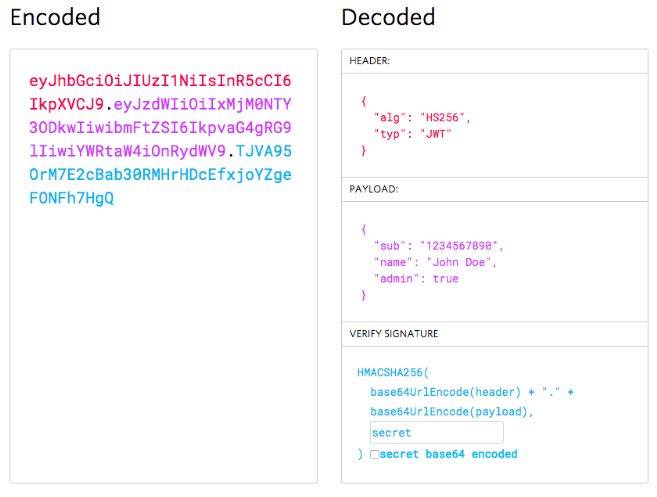
\includegraphics[width=0.6\textwidth]{jwt-beispiel.png}
  
  
\raggedleft
    \footnotesize\sffamily\textbf{Quelle:} \url{https://jwt.io/introduction} am 27. April 2023
  \caption{Beispiel eines verschlüsselten Tokens von JWT}
  \label{fig:jwt-example}
\end{figure}
        \subsubsection{Chakra UI}
        \label{sec:chakraUI}
Chakra UI ist eine simple Komponenten Bibliothek, welche das designen von React Anwendungen vereinfacht\footnote{Quelle: \url{https://chakra-ui.com/} am 22. April 2023}. Es stellt Komponenten zur Verfügung, welchen verschiedene Attribute zugeordnet werden können um diese nach eigenem ermessen zu designen (siehe Code Beispiel \ref{lst:chakra-example} und Abbildung \ref{fig:chakra-example}).


  \begin{figure}[h]
  \centering
  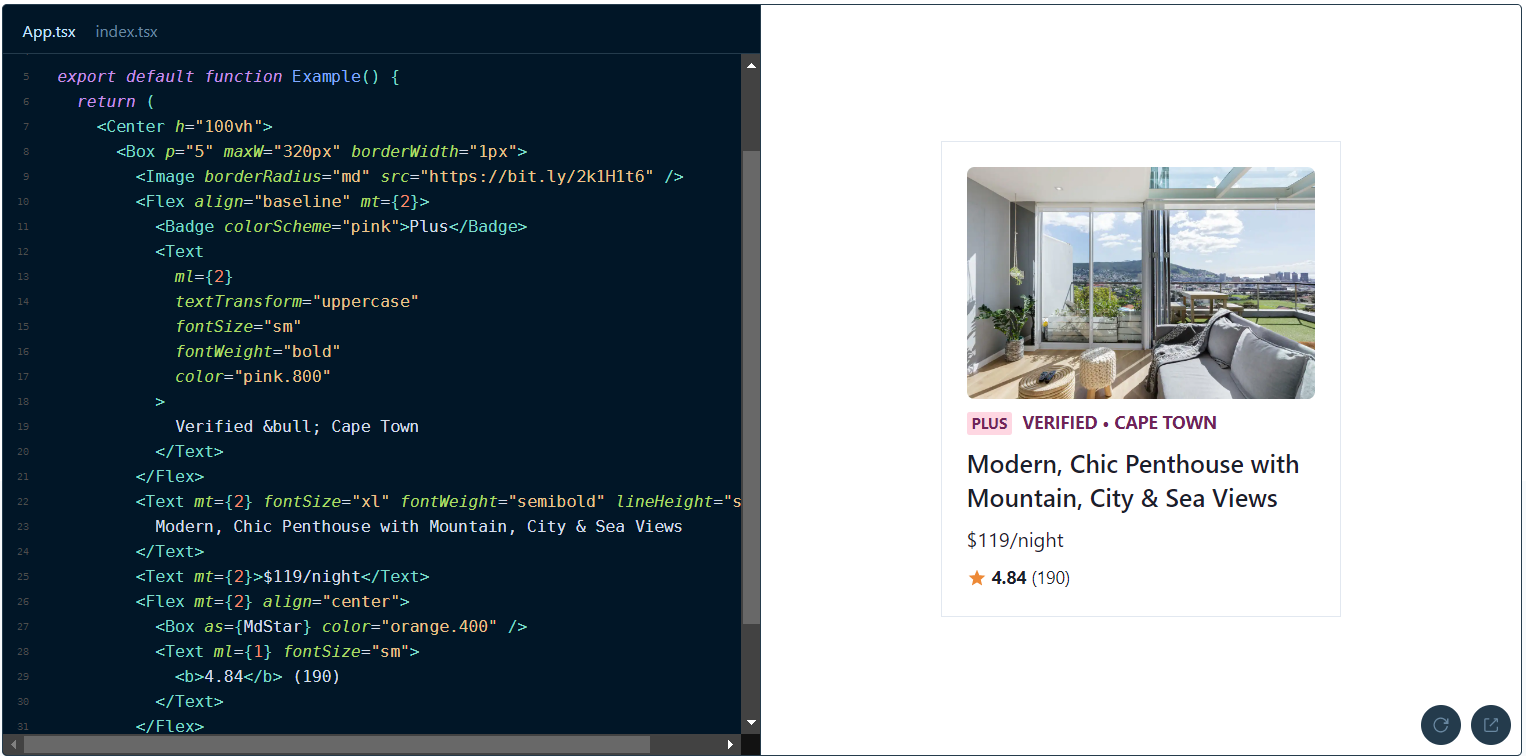
\includegraphics[width=0.4\textwidth]{Chakra-UI Beispiel.png}
  
\raggedleft
    \footnotesize\sffamily\textbf{Quelle:} \url{https://chakra-ui.com/} am 27. April 2023
  \caption{Darstellung der mit Chakra UI designten React Komponente aus dem Code Beispiel \ref{lst:chakra-example}}
  \label{fig:chakra-example}
\end{figure}
  

\begin{lstlisting}[style=codeStyle, caption={Beispiel mit Chakra UI designten React Komponente (siehe Abbildung  \textbf{Quelle:} \url{https://chakra-ui.com/} am 27. April 2023}, label={lst:chakra-example}]
import * as React from "react";
import { Box, Center, Image, Flex, Badge, Text } from "@chakra-ui/react";
import { MdStar } from "react-icons/md";

export default function Example() {
  return (
    <Center h="100vh">
      <Box p="5" maxW="320px" borderWidth="1px">
        <Image borderRadius="md" src="https://bit.ly/2k1H1t6" />
        <Flex align="baseline" mt={2}>
          <Badge colorScheme="pink">Plus</Badge>
          <Text
            ml={2}
            textTransform="uppercase"
            fontSize="sm"
            fontWeight="bold"
            color="pink.800"
          >
            Verified &bull; Cape Town
          </Text>
        </Flex>
        <Text mt={2} fontSize="xl" fontWeight="semibold" lineHeight="short">
          Modern, Chic Penthouse with Mountain, City & Sea Views
        </Text>
        <Text mt={2}>$119/night</Text>
        <Flex mt={2} align="center">
          <Box as={MdStar} color="orange.400" />
          <Text ml={1} fontSize="sm">
            <b>4.84</b> (190)
          </Text>
        </Flex>
      </Box>
    </Center>
  );
}
\end{lstlisting}
        \subsubsection{Formik und Yup}
        \label{sec:formik}
Formik ist die beliebteste Open-Source-Bibliothek für Formulare in React \footnote{Quelle: \url{https://formik.org/} am 22. April 2023}. Sie vereinfacht die Handhabung von Formularen und bietet Funktionen wie Validierung der eingegebenen Werte, Fehlermeldungen und Unterstützung für mehrstufige Formulare.

Yup ist eine Bibliothek  zur einfachen Definition von Schemata, die von bestimmten Formularen erfüllt werden sollen. Sie ermöglicht die Erstellung komplexer Schemata mit wenig Code\footnote{Quelle: \url{https://github.com/jquense/yup} am 22. April 2023}.

Die Integration von Yup-Schemata in Formik-Formularen ist bereits unterstützt, was eine einfache Handhabung von Überprüfungen und Fehlerbehandlungen bei Benutzereingaben ermöglicht.

        \subsubsection{chess.js}
        \label{sec:chess.js}
chess.js ist eine Schach Bibliothek, welche die gesamte Schachlogik zur Verfügung stellt\footnote{Quelle: \url{https://github.com/jhlywa/chess.js/} am 22. April 2023}. Es bietet Methoden, welche alle aktuell möglichen Züge ausgibt, einen Zug ausführt und verschiedene Notationen des Zuges zurückgibt, überprüft ob es sich um ein Schachmatt oder Patt handelt, eine Partie mittels einer FEN\footnote{Quelle: \url{https://de.wikipedia.org/wiki/Forsyth-Edwards-Notation} am 22. April 2023} oder PGN\footnote{\url{https://de.wikipedia.org/wiki/Portable_Game_Notation} am 22. April 2023} Notation laden kann und vieles weitere. 
        \subsubsection{chessground}
        \label{sec:chessground}
chessground ist ein Open-Source-Schach-User-Interface, das ursprünglich für die Online-Schachplattform \url{lichess.org} entwickelt wurde\footnote{Quelle: \url{https://github.com/lichess-org/chessground} am 22. April 2023}. Es bietet zahlreiche Konfigurationsmöglichkeiten, wie zum Beispiel Animationen beim bewegen von Figuren, Auswahl der anklickbaren und bewegbaren Figuren, Anpassung des Figurendesigns und vieles mehr. Die eigentliche Schachlogik ist nicht enthalten, sodass verschiedene Schachvarianten mit Sonderregelungen implementiert werden können.

\subsubsection{bcrypt}
\label{sec:bcrypt}
bcrypt ist eine Bibliothek welche entwickelt wurde um Passwörter zu verschlüsseln. Es basiert auf Blowfish, einem Verschlüsselungsalgorithmus, und löst das Problem, dass durch schnellere Hardware Passwörter immer schneller kodiert und dekodiert werden können und dadurch Sicherheitsrisiken entstehen. Es löst dieses Problem dadurch, dass es die Passwörter um einen selbst definierbaren Faktor zeitlich länger kodiert indem es mehrere Iterationen durchführt\footnote{Quelle: \url{https://auth0.com/blog/hashing-in-action-understanding-bcrypt/}}.
        